% !TeX root = ..\main.tex
\section{Thiết kế lược đồ BPMN}

% !TeX root = ..\main.tex
\section{Thiết kế lược đồ BPMN}

\subsection{Khách hàng mua hàng trực tiếp}
\begin{figure}[!htp]
    \centering
    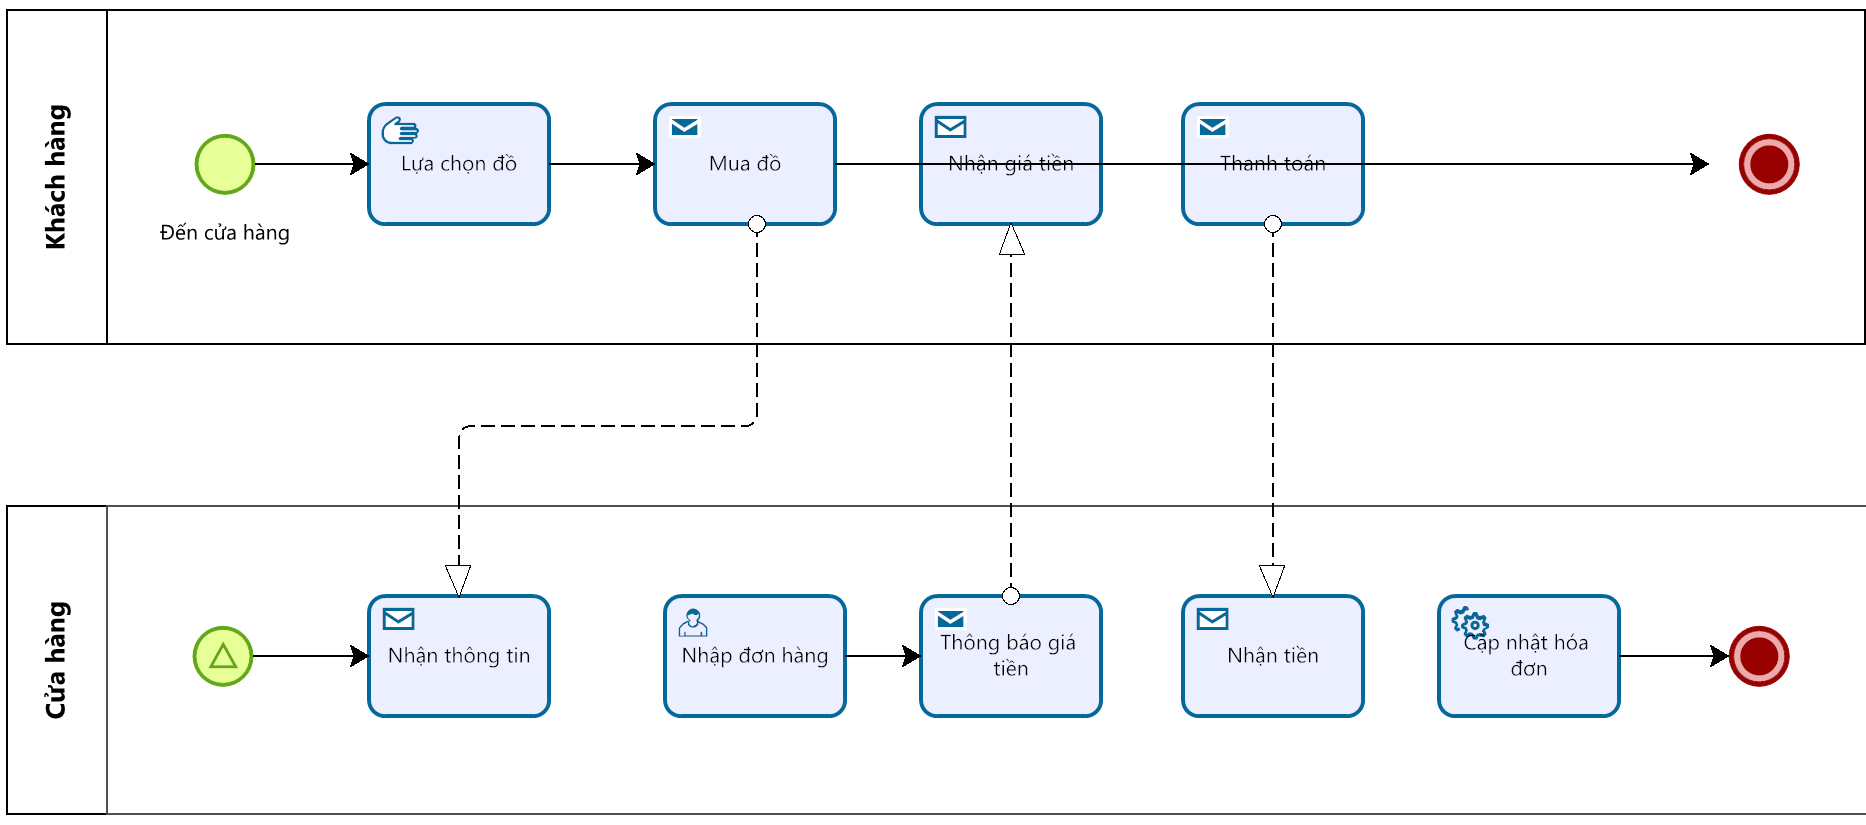
\includegraphics[width=14cm]{img/BPMN/Hien/Customer_buyOffline.png}
    \newline
    \caption{Lược đồ BPMN cho quy trình khách hàng mua hàng trực tiếp}
\end{figure}

\subsection{Đăng nhập}
\begin{figure}[!htp]
    \centering
    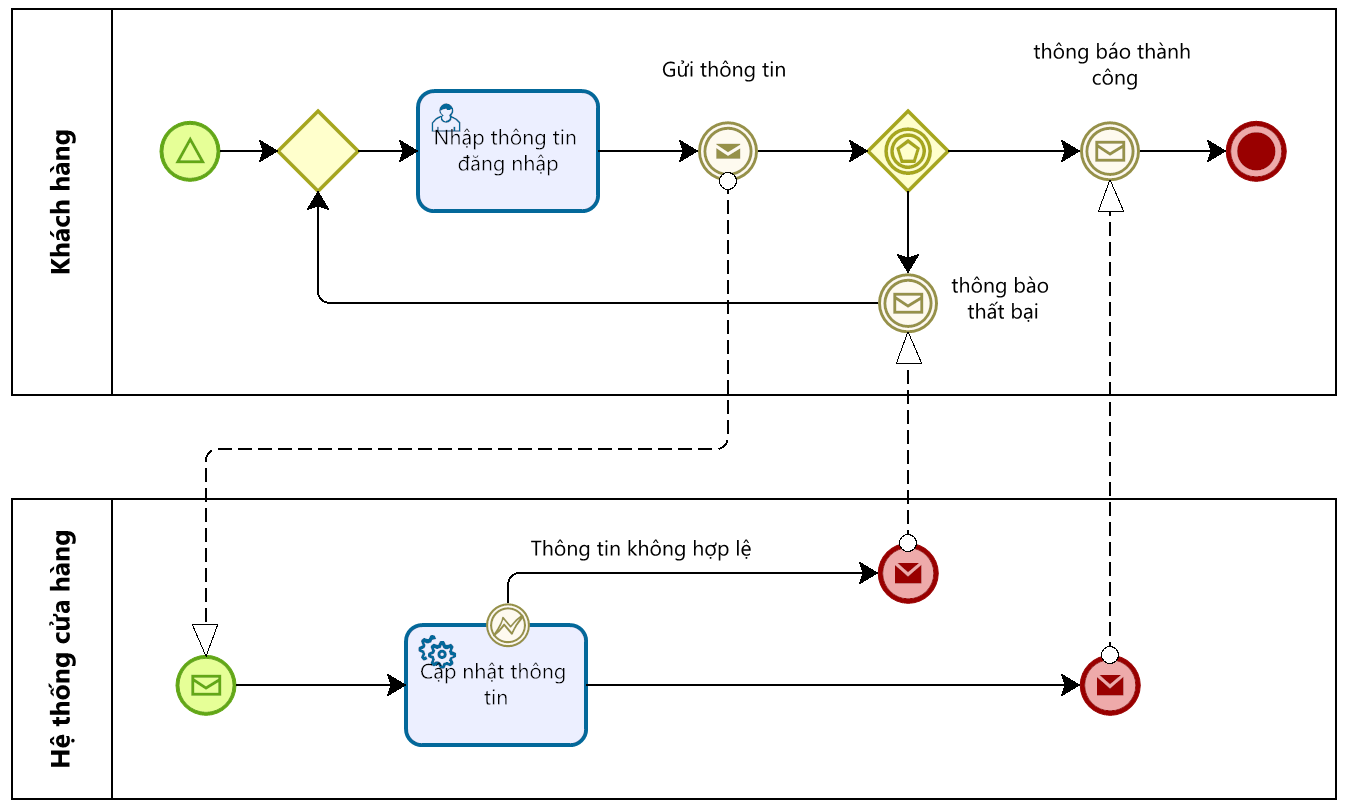
\includegraphics[width=14cm]{img/BPMN/Hien/Customer_login.png}
    \newline
    \caption{Lược đồ BPMN cho quy trình đăng nhập}
\end{figure}

\subsection{Đăng ký tài khoản}
\begin{figure}[!htp]
    \centering
    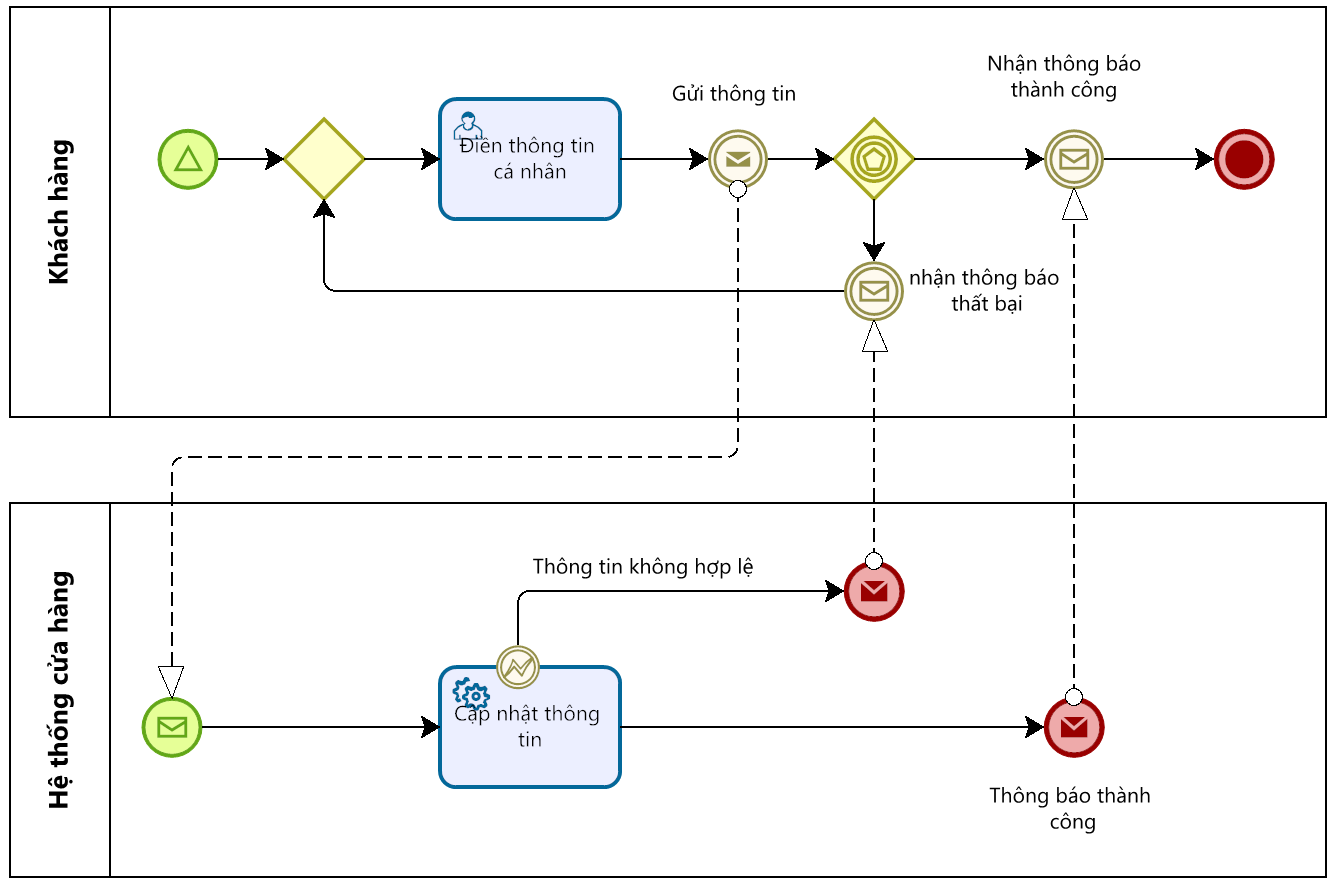
\includegraphics[width=14cm]{img/BPMN/Hien/Customer_register.png}
    \newline
    \caption{Lược đồ BPMN cho quy trình đăng ký tài khoản mới}
\end{figure}


\subsection{Làm mới mật khẩu}
\begin{figure}[!htp]
    \centering
    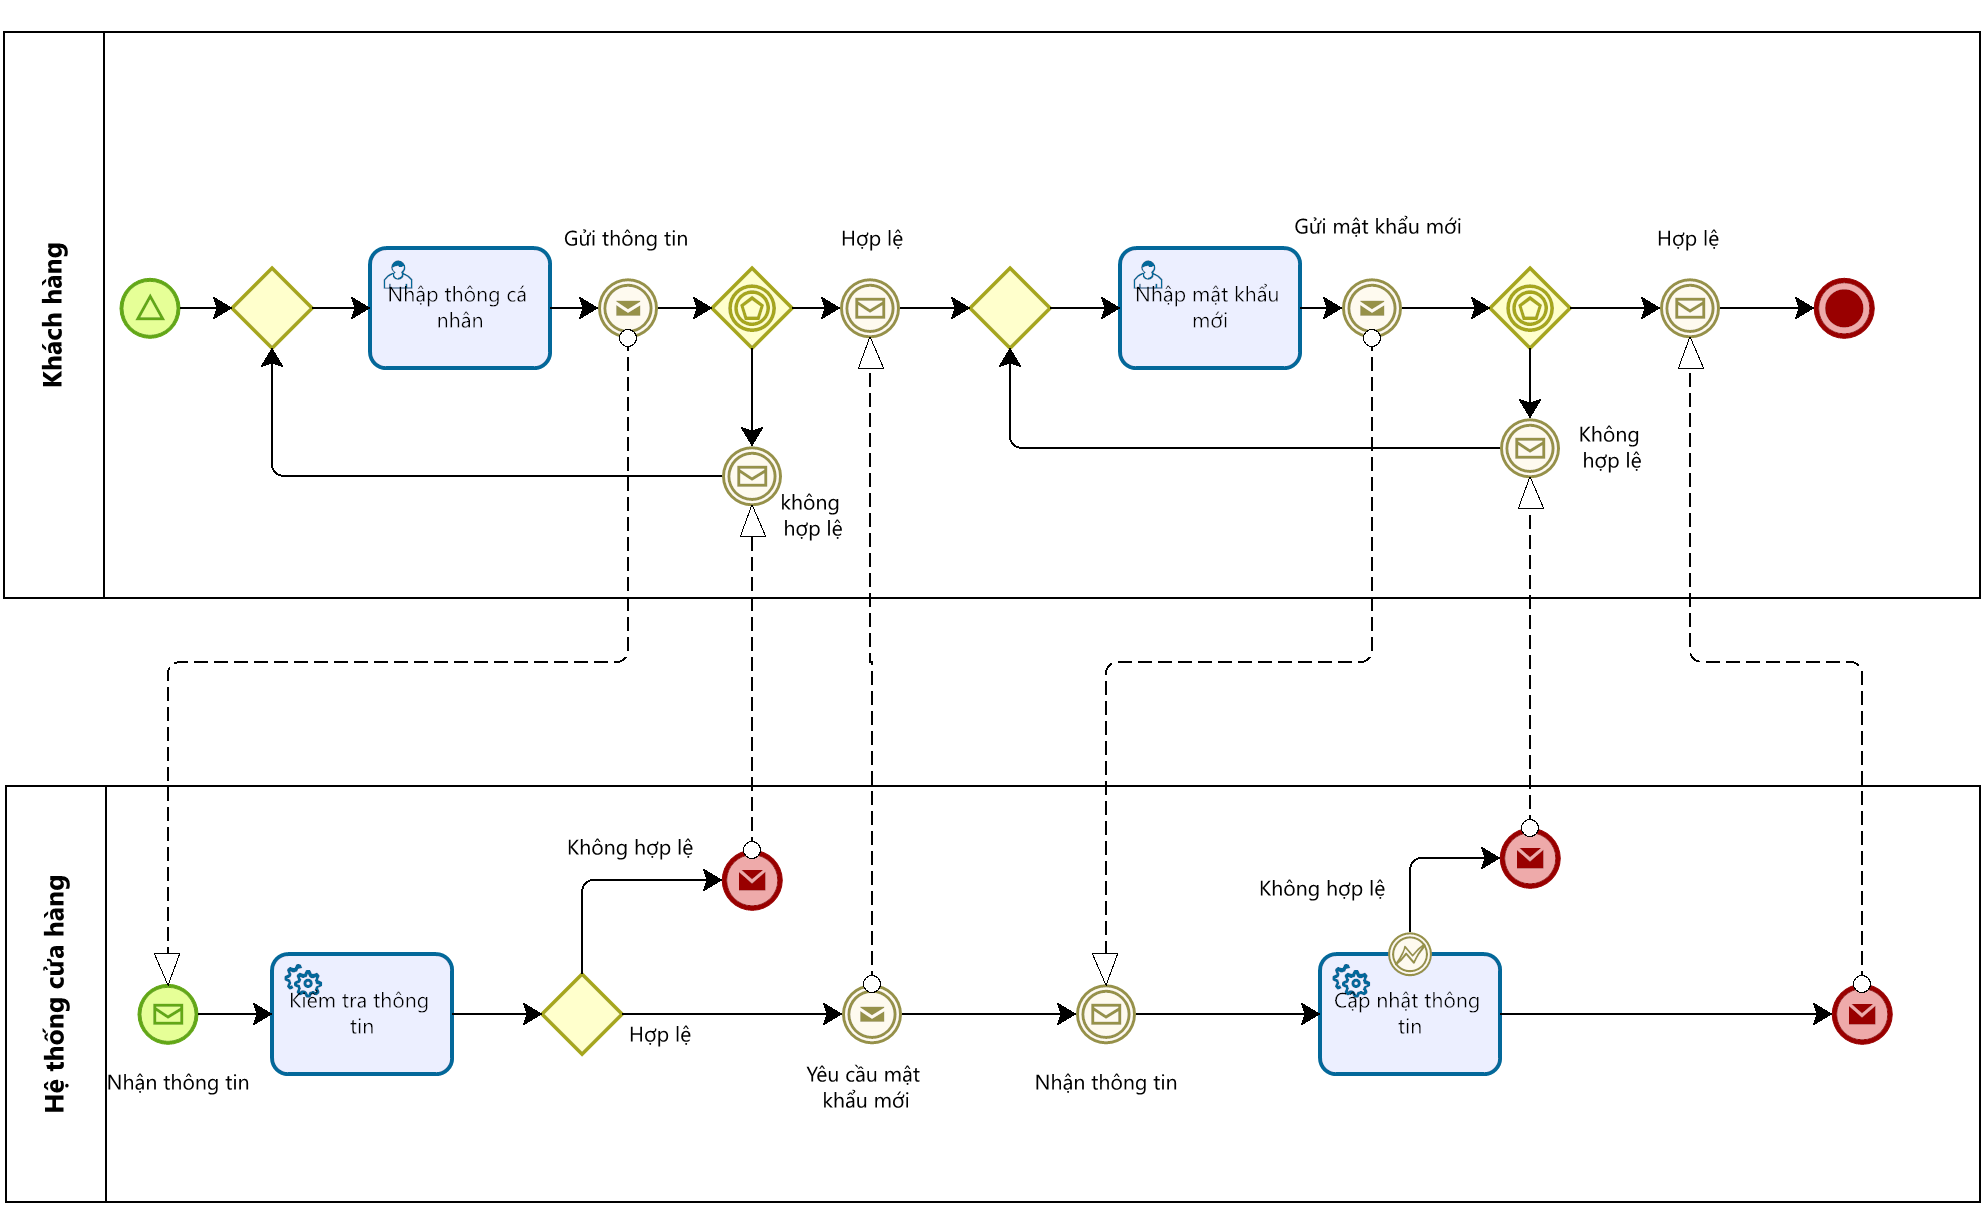
\includegraphics[width=14cm]{img/BPMN/Hien/Customer_resetPassword.png}
    \newline
    \caption{Lược đồ BPMN cho quy trình làm mới mật khẩu}
\end{figure}



\subsection{Quản lý chi nhánh}
\begin{figure}[!htp]
    \centering
    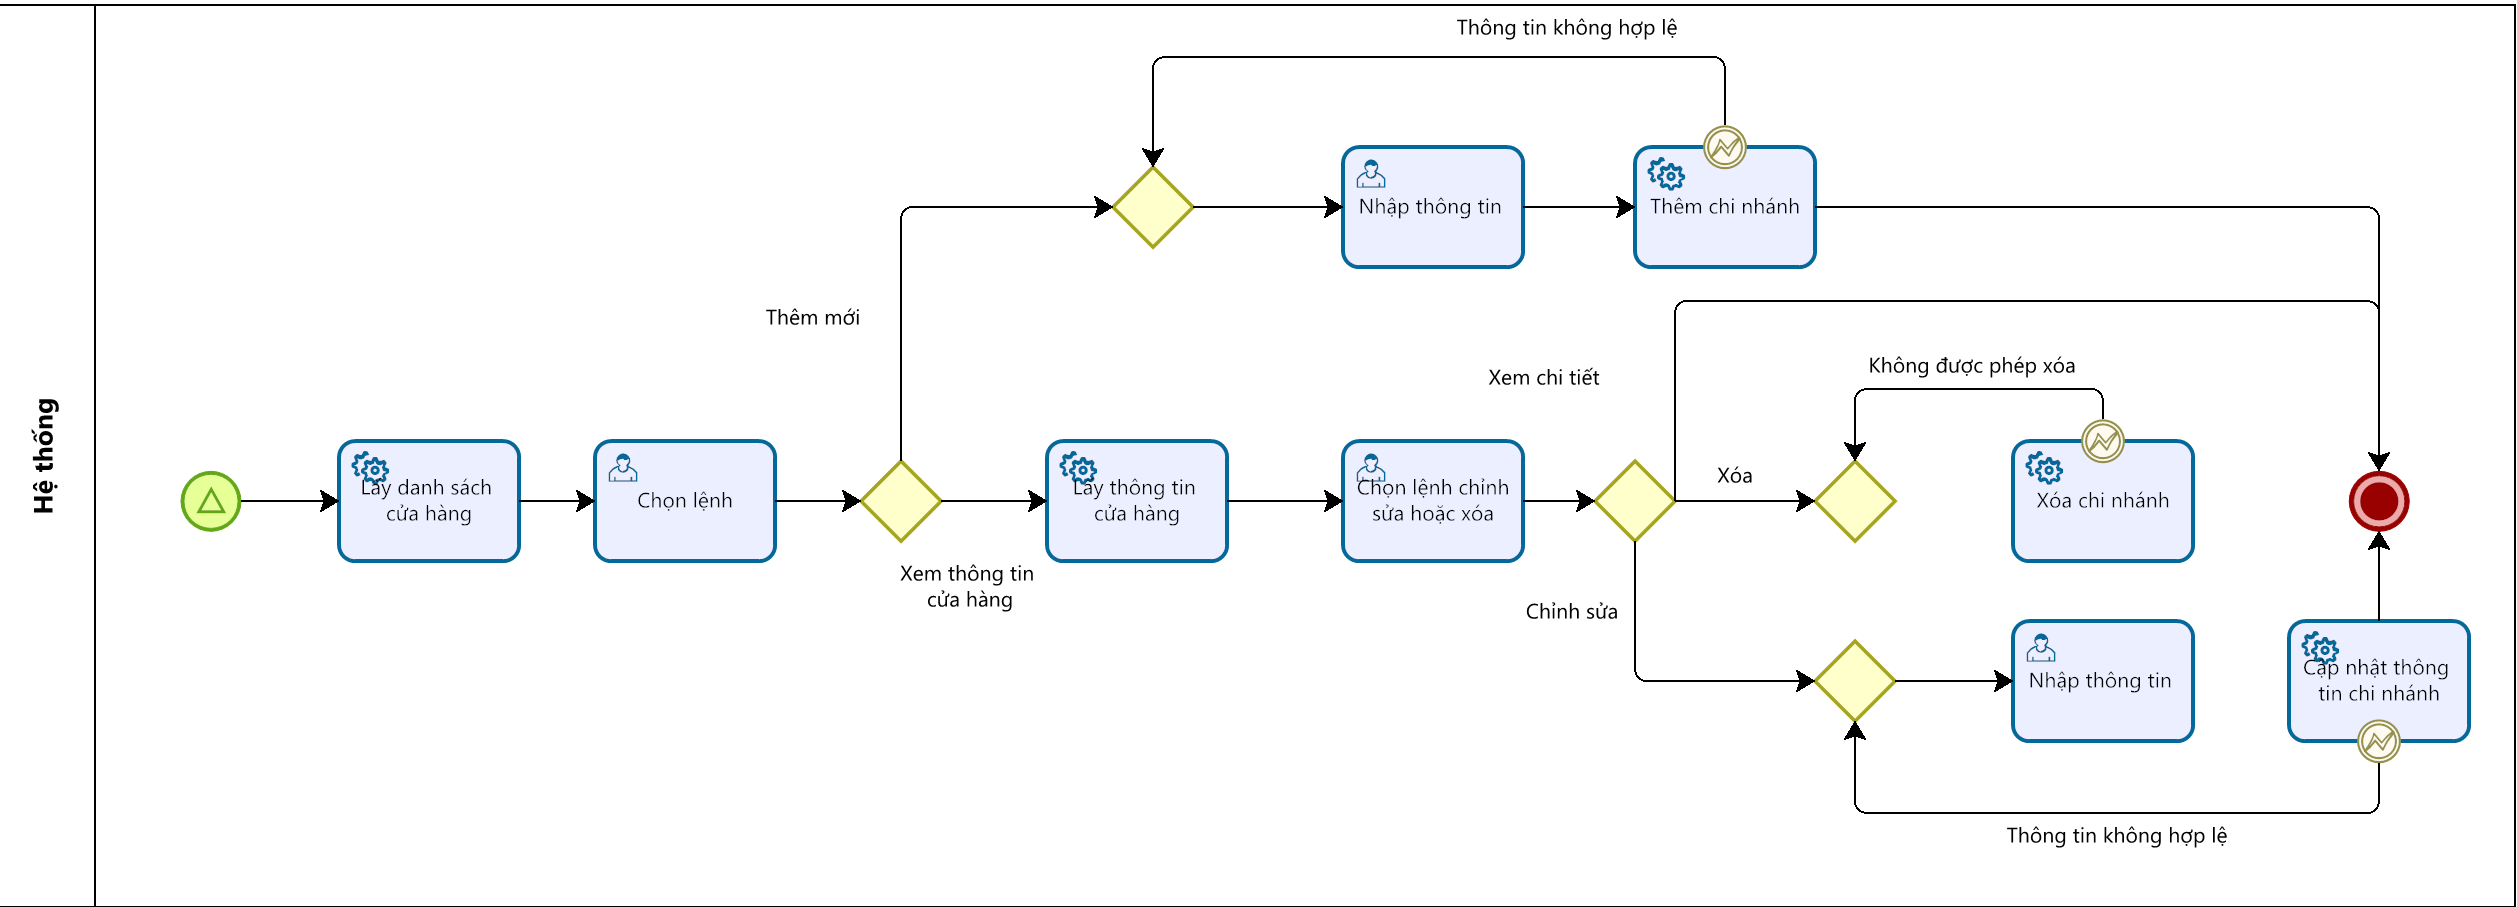
\includegraphics[width=14cm]{img/BPMN/Hien/Branch_management.png}
    \newline
    \caption{Lược đồ BPMN cho quy trình quản lý chi nhánh}
\end{figure}


\subsection{Quản lý nhân viên}
\begin{figure}[!htp]
    \centering
    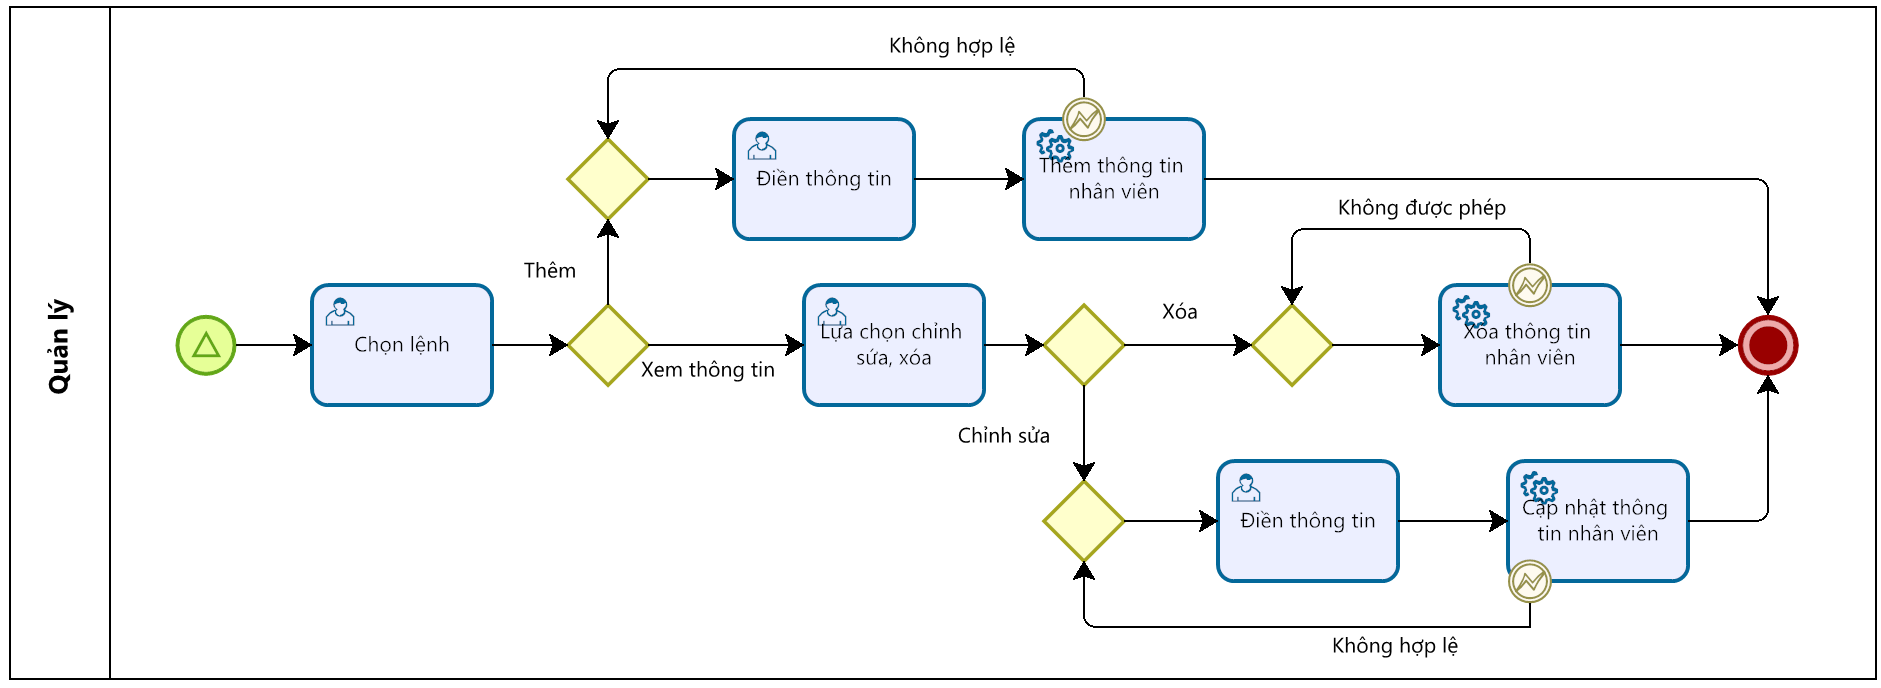
\includegraphics[width=14cm]{img/BPMN/Hien/Employee_Management.png}
    \newline
    \caption{Lược đồ BPMN cho quy trình quản lý nhân viên}
\end{figure}

\subsubsection*{Tạo yêu cầu thêm, xóa nhân viên}
\begin{figure}[!htp]
    \centering
    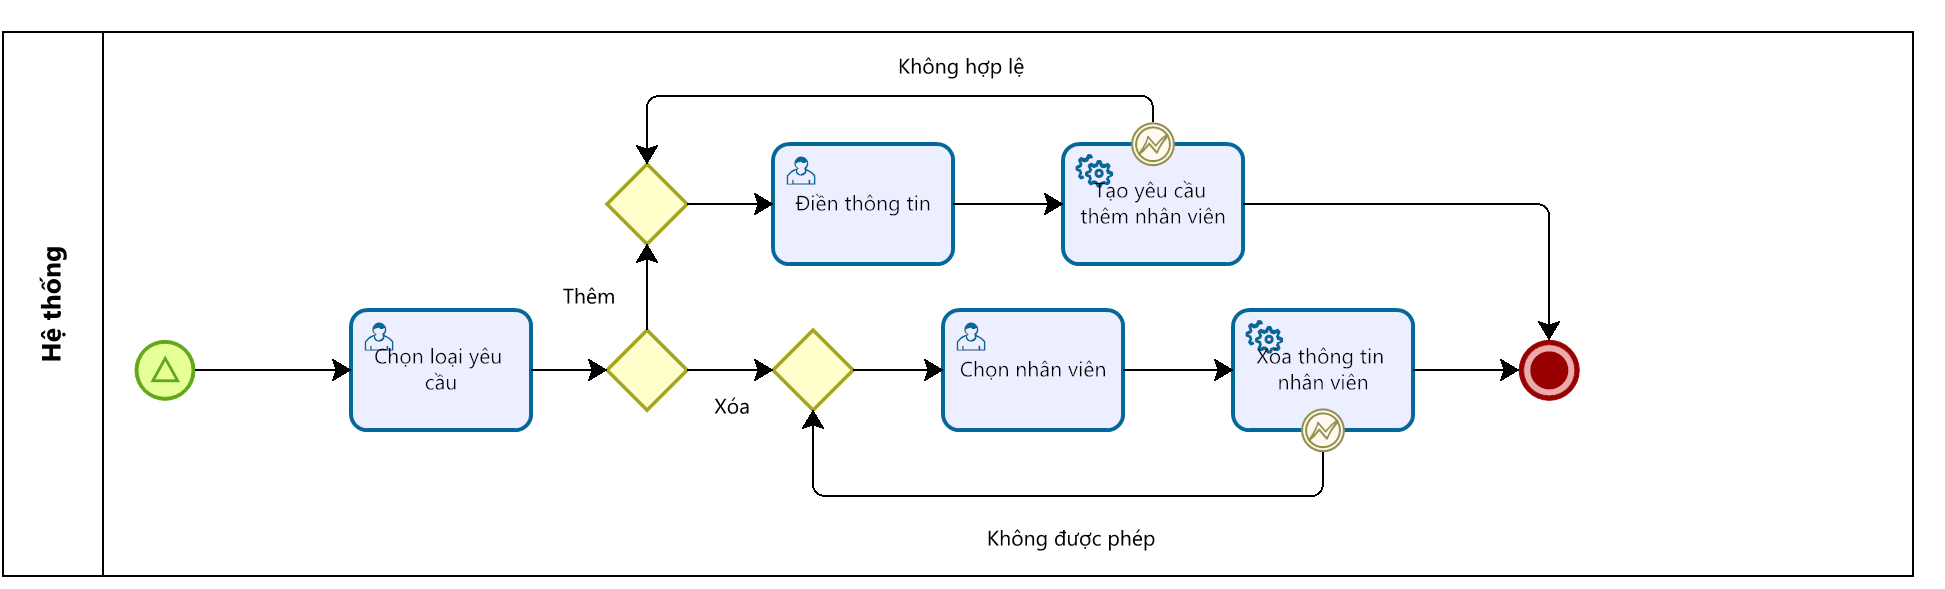
\includegraphics[width=14cm]{img/BPMN/Hien/Employee_request.png}
    \newline
    \caption{Lược đồ BPMN cho quy trình quản lý nhân viên}
\end{figure}

